\section{Optimization Results}
\label{sec:optimization_plots}

Training performance over optimization trials are plotted below for one run for each task and method combination. The figures can be seen below for ScoNe (Figure~\ref{fig:scone_plots}), HotPotQA (Figure~\ref{fig:hotpotqa_plots}), HoVer (Figure~\ref{fig:hover_retrieve30_discrete_plots}), HotPotQA conditional (Figure~\ref{fig:hotpotqa_conditional_plots}), Iris (Figure~\ref{fig:iris_plots}), and Heart Disease (Figure~\ref{fig:heart_disease_plots}).

\begin{figure*}[ht]
  \centering
  \includegraphics[width=1.0\textwidth]{figures/scone_plots.pdf}
  \caption{ScoNe optimization results.}
  \label{fig:scone_plots}
\end{figure*}

\begin{figure*}[ht]
  \centering
  \includegraphics[width=1.0\textwidth]{figures/hotpotqa_plots.pdf}
  \caption{HotPotQA optimization results.}
  \label{fig:hotpotqa_plots}
\end{figure*}

\begin{figure*}[ht]
  \centering
  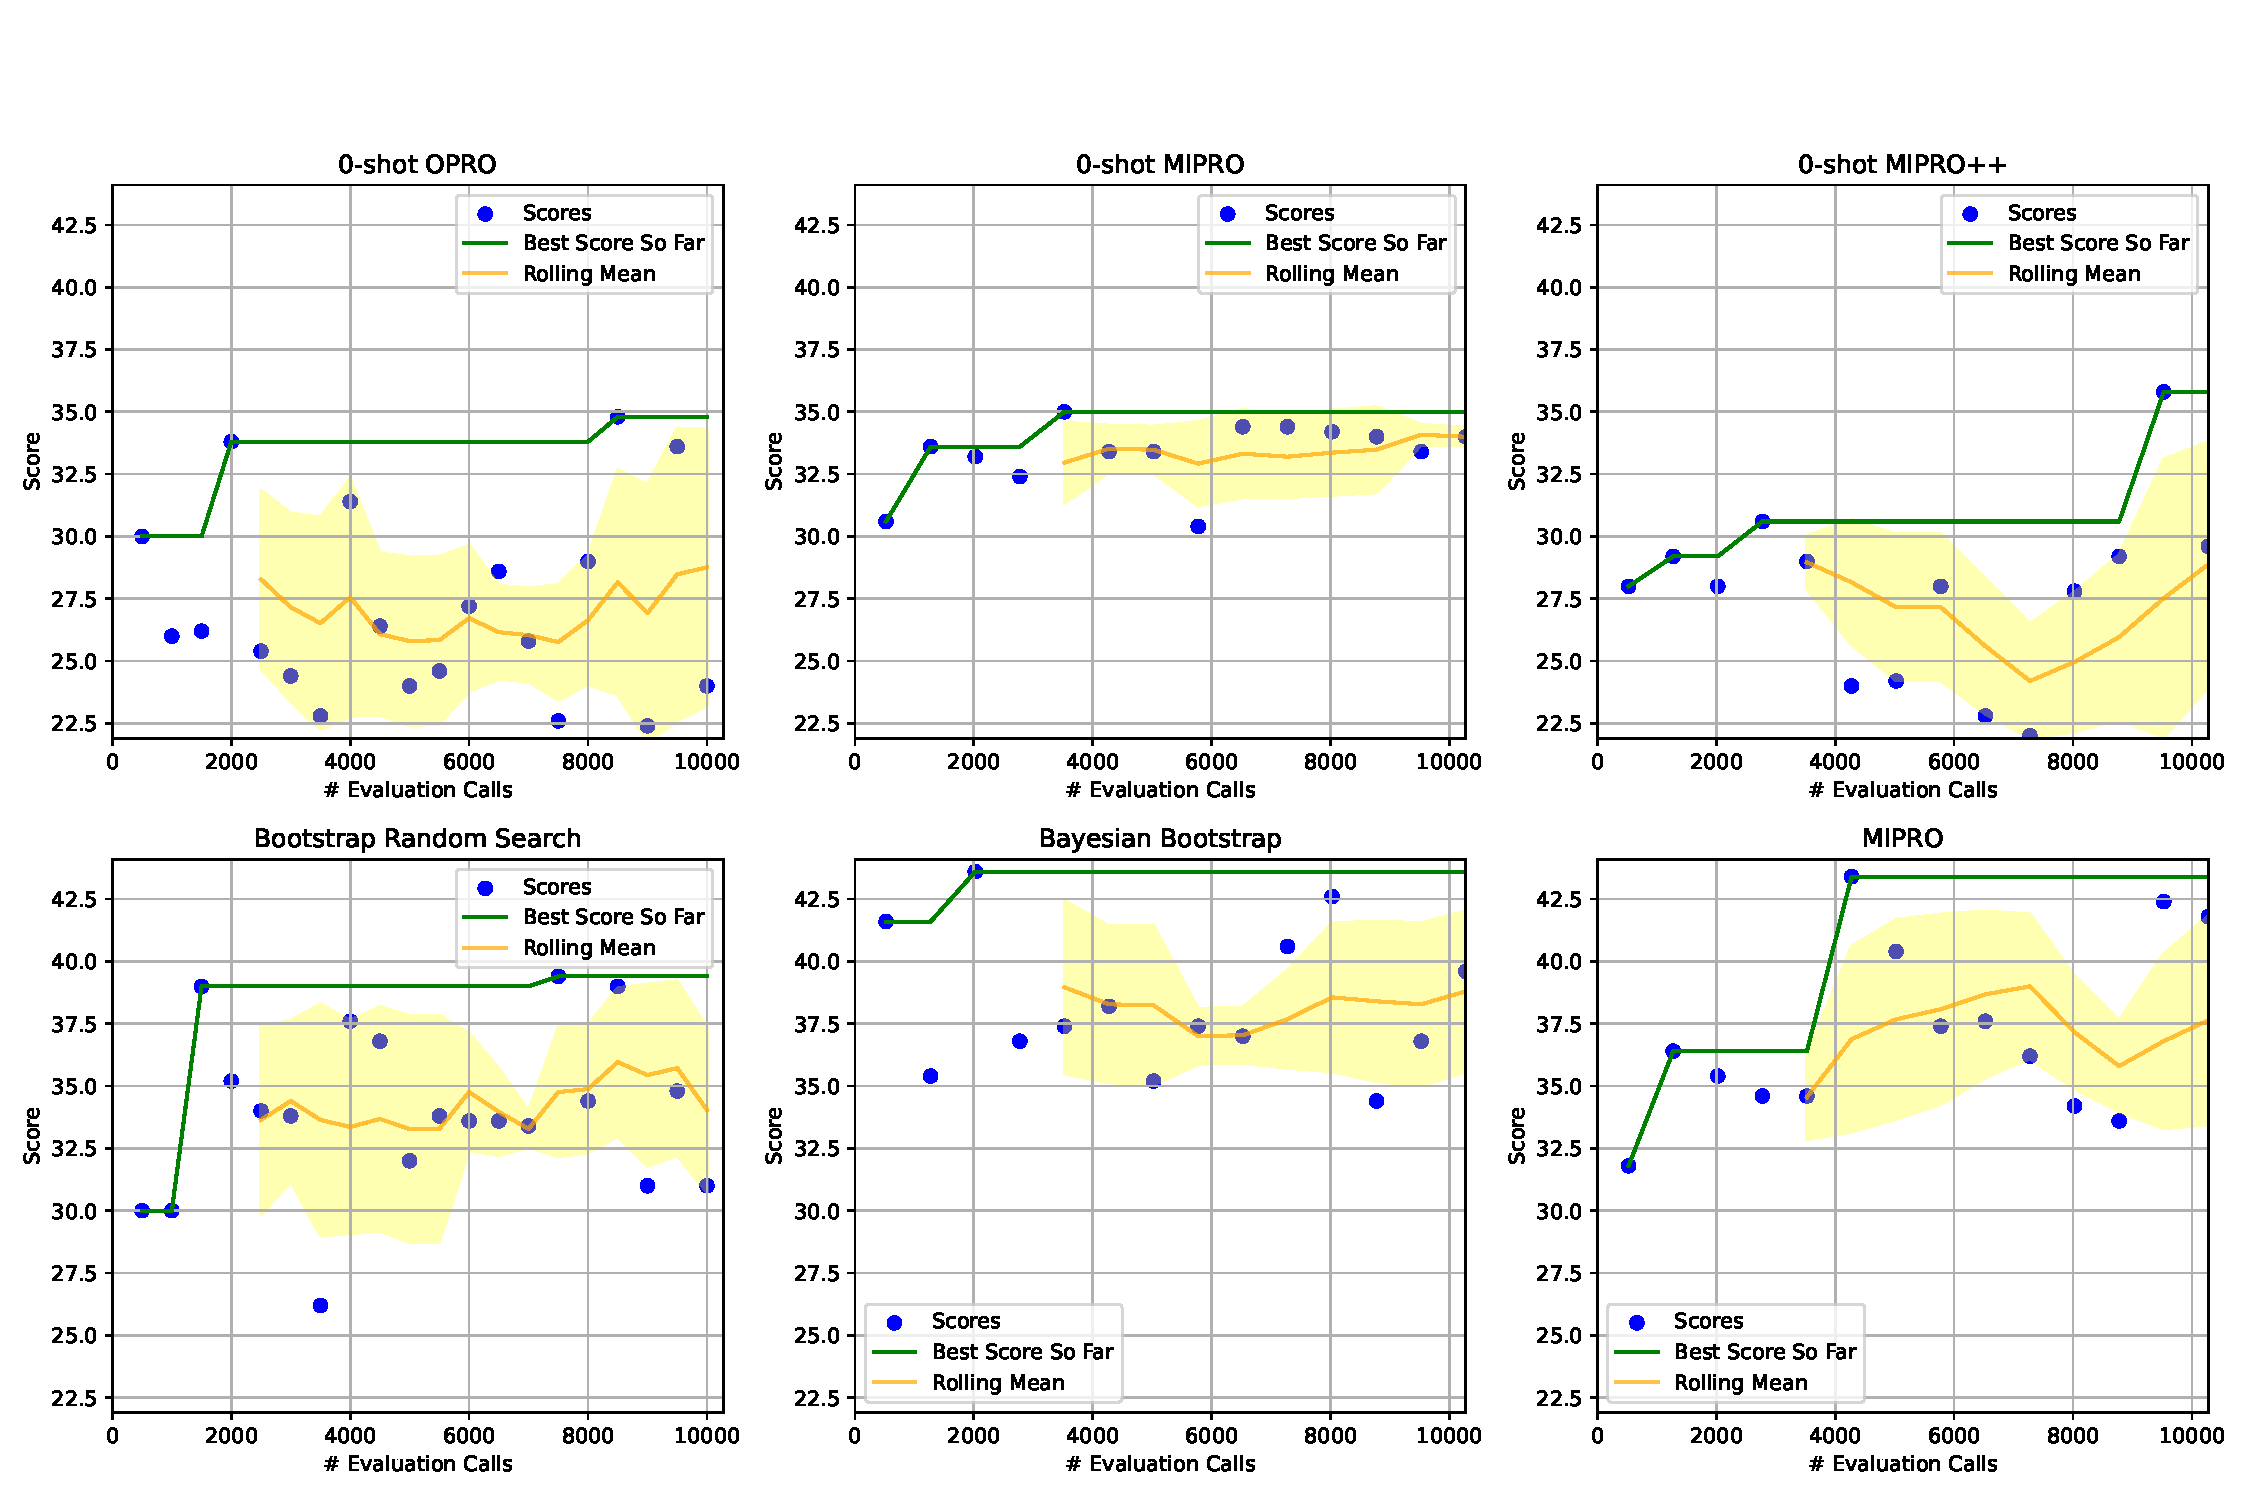
\includegraphics[width=1.0\textwidth]{figures/hover_retrieve30_discrete_plots.pdf}
  \caption{HoVer optimization results.}
  \label{fig:hover_retrieve30_discrete_plots}
\end{figure*}

\begin{figure*}[ht]
  \centering
  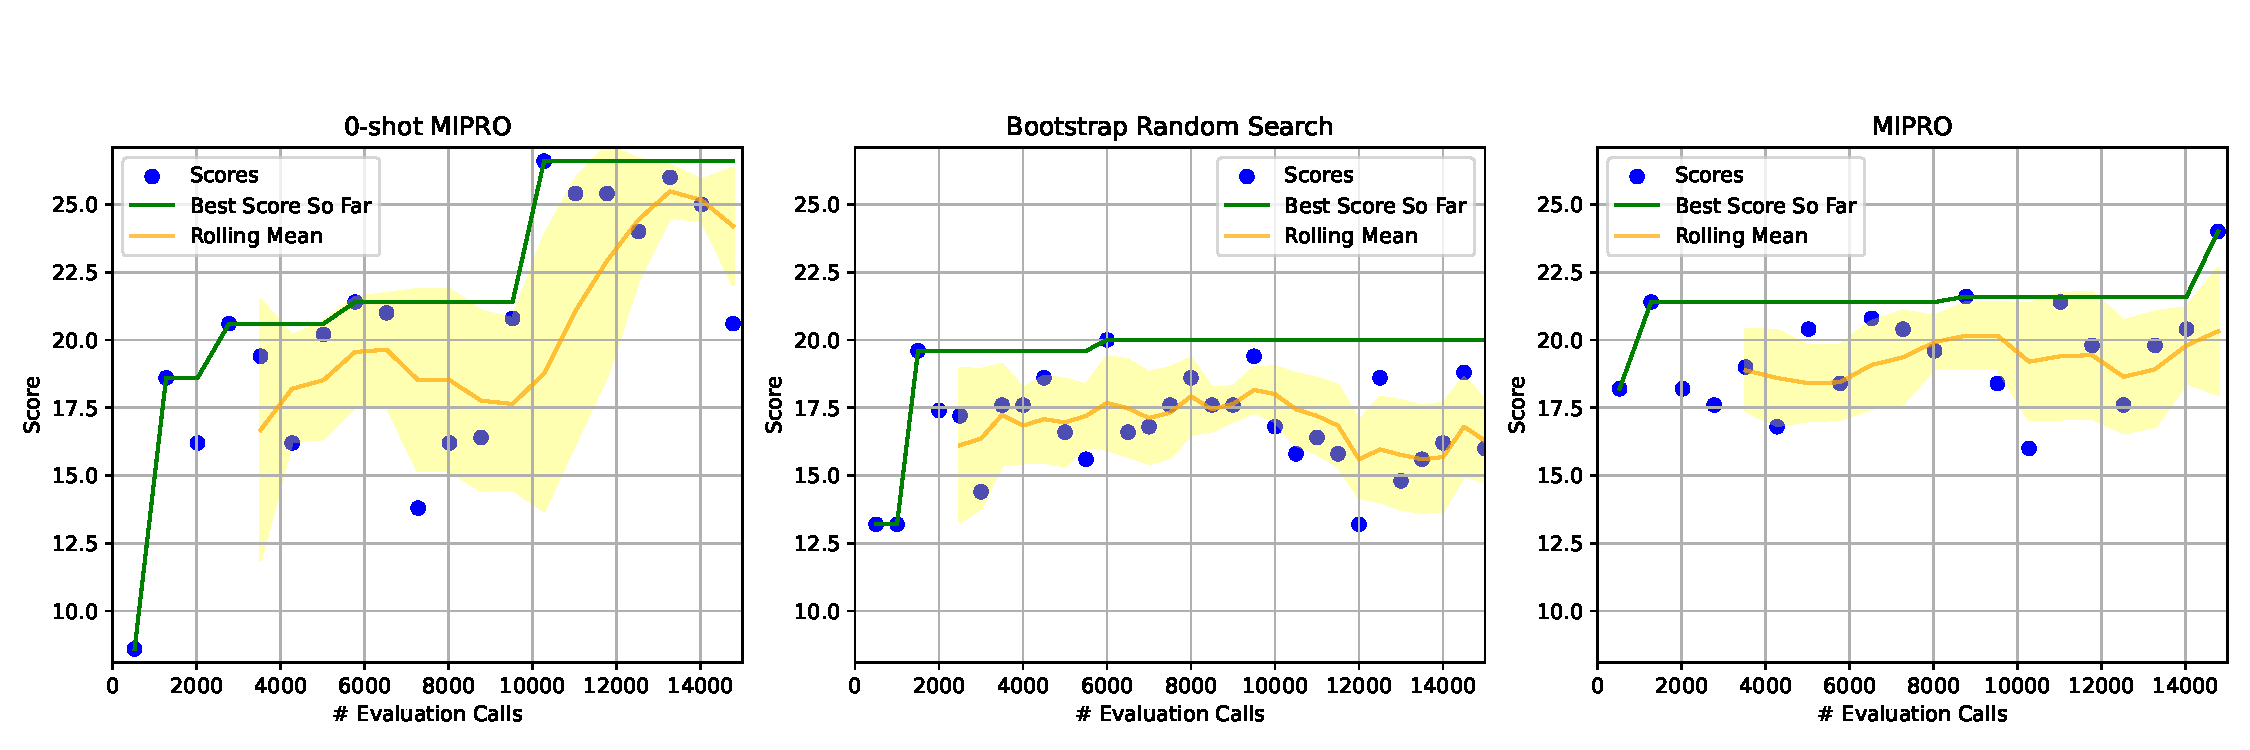
\includegraphics[width=1.0\textwidth]{figures/hotpotqa_conditional_plots.pdf}
  \caption{HotPotQA Conditional optimization results.}
  \label{fig:hotpotqa_conditional_plots}
\end{figure*}

\begin{figure*}[ht]
  \centering
  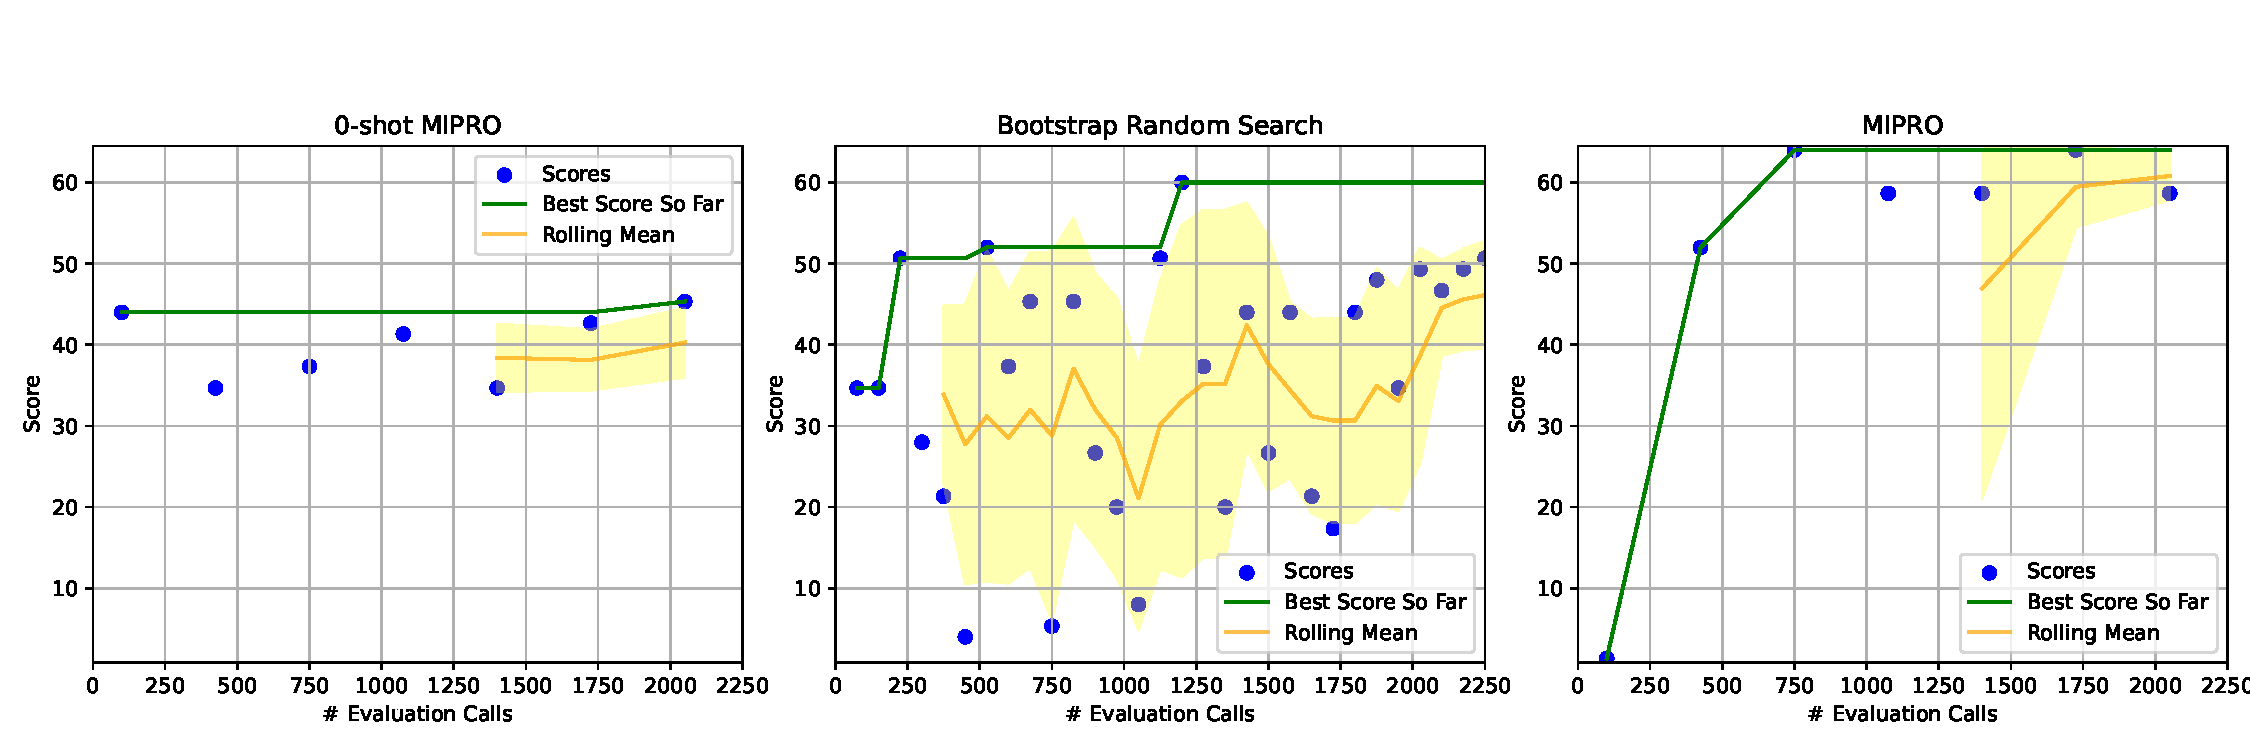
\includegraphics[width=1.0\textwidth]{figures/iris_plots.pdf}
  \caption{Iris-Typo optimization results. Plots from run where the default prompt spelled "versicolor" as "versicolour".}
  \label{fig:iris_plots}
\end{figure*}

\begin{figure*}[ht]
  \centering
  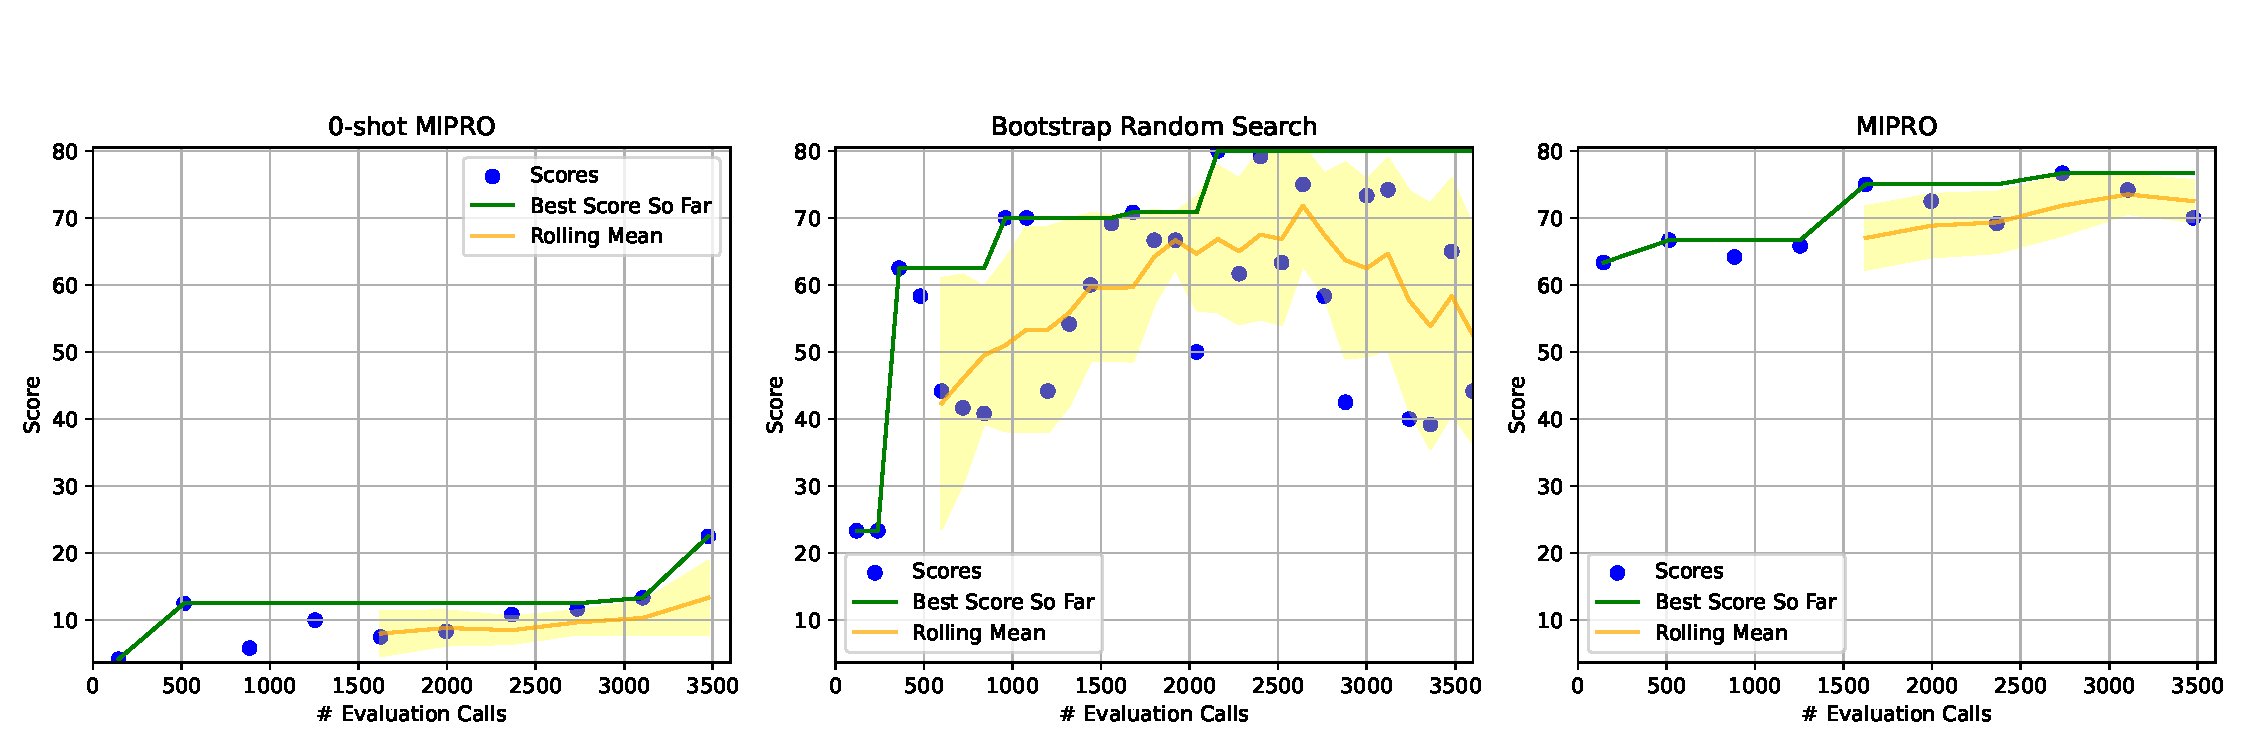
\includegraphics[width=1.0\textwidth]{figures/heart_disease_plots.pdf}
  \caption{Heart Disease optimization results.}
  \label{fig:heart_disease_plots}
\end{figure*}
